% !TeX spellcheck = en_US
\chapter{Using RDF-specific Features}\label{ch:rdfSpecificFeatures}

GRP is a compressor made for all kinds of graphs. This also means that it is not specially adapted for RDF. It is therefore possible to use some special features of RDF to achieve a better compression ratio. This is what chapter~\ref{sec:ontKnowledge} will deal with.

On the other hand, chapter~\ref{ch:GRPvsHDT} already revealed that most of the compressed size is determined by the dictionary, since saving the dictionary is more complex than saving the graph structure. Chapter~\ref{sec:dictFeatures} will therefore focus on how to compress the dictionary even more.

\section{Ontology Knowledge}\label{sec:ontKnowledge}

RDF has meta data that contains background knowledge about the actual data. This is also called ontology. An ontology is normally itself an RDF graph. There are two known languages for formulating an ontology: RDFS~\footnote{\label{foot:3}https://www.w3.org/TR/rdf-schema/} and OWL~\footnote{\label{foot:4}https://www.w3.org/TR/2012/REC-owl2-overview-20121211/\#Documentation\_Roadmap}. Of these, OWL is the more powerful and is therefore chosen here.

This chapter is about finding out whether one can change the structure of an RDF graph by applying knowledge from its ontology so that it is more compressible for GRP, but at the same time remains semantically equivalent to the original graph. In this way no data would be lost by compression.

In Ch.~\ref{ch:GRPvsHDT} it has already been mentioned that GRP depends more on the structure of the input graph than HDT does. It will therefore be interesting to see how applying ontology knowledge influences GRP's compression ratio.


\subsection{Theory}

\subsection{Evaluation}

\section{Dictionary Features}\label{sec:dictFeatures}

As already seen in Ch.~\ref{ch:GRPvsHDT}, the dictionary makes up most of the memory of a compressed RDF graph. It is therefore worth investigating whether the dictionary can be compressed better. One can take advantage of certain features of the dictionary to achieve that.

\subsection{Theory}

As mentioned above, GRP does not have its own method for compressing the dictionary. We have therefore taken the compression method from HDT, and applied it in GRP to ensure a fair comparison.

HDT has a fairly mature mechanism for compressing the dictionary.\todo{genauer erklären}

\subsubsection{Literals}

Objects in RDF can be literals. Literals typically contain constant values and usually have no common prefixes. Therefore the compression of HDT is not suitable for these. Since literals can often contain whole flow texts, a text compression would probably be well applicable. An example of such a text compression is a Huffman Code~\cite{huffman}. Here the text is converted into a binary format. Every single character of a text is binary coded, whereby frequently occurring characters get short and rare characters get longer codes. These codes are expressed by a binary Huffman tree. An example can be seen in Fig.~\ref{fig:huffmantree}. Each leaf contains a symbol whereas the one and zeros on the path to the symbol define its code. The tree is constructed in such a way that paths to frequent characters are shorter than those to rare characters. The whole procedures can be seen in~\cite{huffman}.

This tree must then be stored in addition to the compressed data so that the original data can be recovered. There is no standard way for storing the binary tree. One approach can be seen in Algorithm~\ref{alg:HuffmanEncode} which has to be started with the root node. That method created an unambiguous bit representation of the tree, since each node has either two or no children.

\begin{algorithm}
	\caption{EncodeNode (TreeNode node)}\label{alg:HuffmanEncode}
	\begin{algorithmic}[1]
		\If{node is leaf}
			\State writeBit(1)
			\State writeCharacter(node.character)
		\Else
			\State writeBit(0)
			\State EncodeNode(node.leftChild)
			\State EncodeNode(node.rightChild)
		\EndIf
	\end{algorithmic}
\end{algorithm}

\begin{figure}
	\centering
	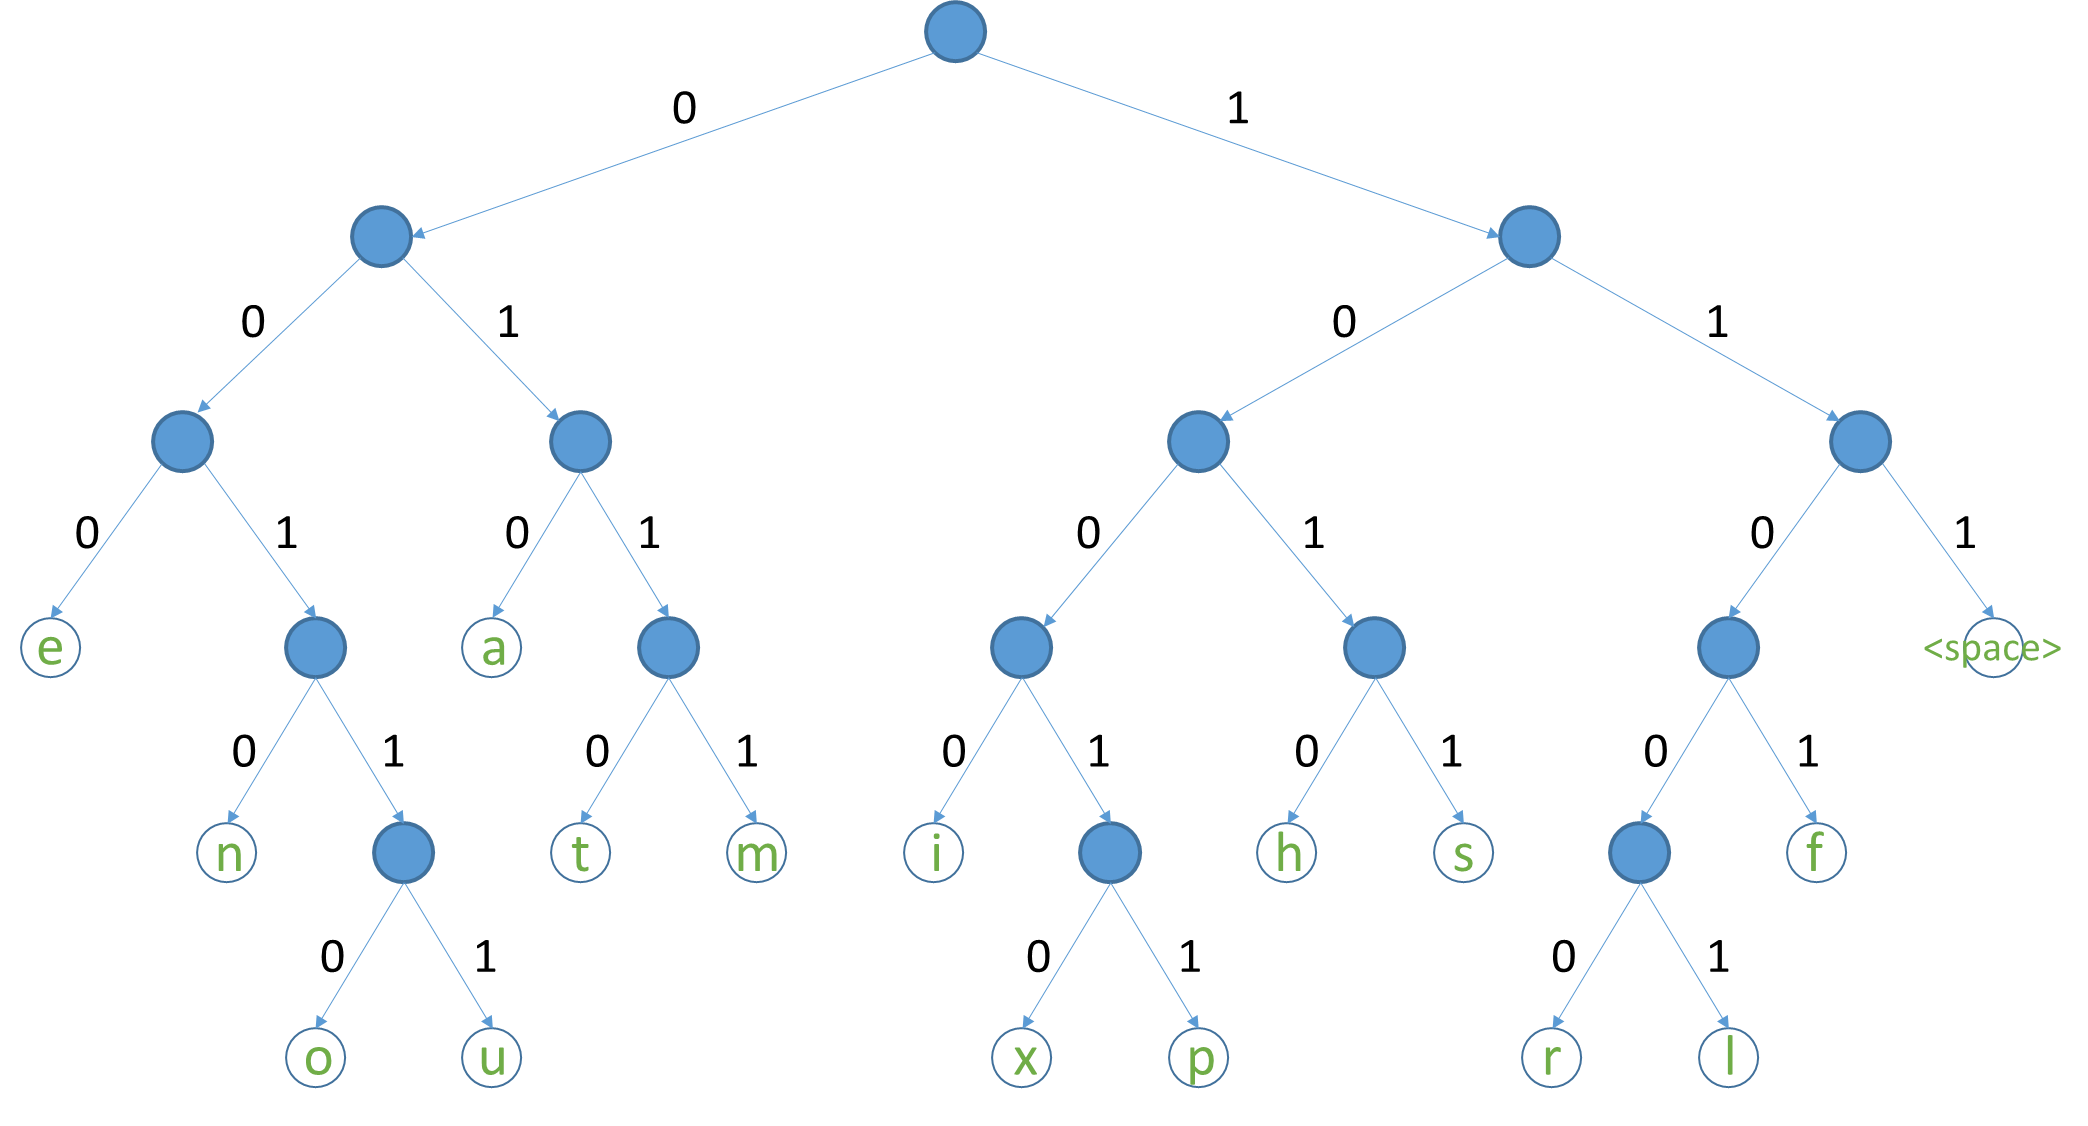
\includegraphics[width=0.9\linewidth]{figures/4_rdf_specific_features/huffman}
	\caption{An example of a Huffman Tree.}
	\label{fig:huffmantree}
\end{figure}


Alternatively, there are pre-computed Huffman trees for natural languages such as English. There they have already investigated which letter occurs how often in English texts and in this way a generally valid Huffman code has been established. The advantage is that one does not have to save the Huffman tree and does not have to calculate it oneself, which saves runtime. The disadvantage, however, is that the tree is not optimal for the text to be compressed, as it is more general. Another problem in our case is that the literals contain a lot of special characters that are not taken into account in prefabricated Huffman codes. This is shown in more detail in Ch.~\ref{sec:evalDict}. Also, it will turn out that saving the Huffman tree does not require much additional memory. Also, the calculation of the tree does not slow down the algorithm significantly. For these reasons we will calculate the Huffman code ourselves to compress the literals. All literals of the input graph are traversed in order to compute the character frequencies.

\subsubsection{Blank Nodes}










\subsection{Evaluation}\label{sec:evalDict}



